\section{Ejercicio 2 - B}
\subsection{Interpretación del enunciado}
Para este ejercicio se pide, dada una red de servidores, los cuales están todos interconectados entre sí con un conjunto de enlaces de costo mínimo; encontrar un servidor tal que, al designarlo $master$ de la red, se garantice que el broadcast se complete en el menor tiempo posible. Vale destacar que este problema toma como entrada la salida del anterior.

Veamos algunos ejemplos. Si consideramos la solución propuesta anteriormente, tenemos que la misma es el siguiente árbol:

\begin{center}
\begin{dot2tex}
graph graphname{
	rank=same;
	rankdir="LR";
	splines=line;
	{rank=same; 1 5}
	{rank=same; 2 6}
	{rank=same; 3 7}
	{rank=same; 4 8}
	1 -- 2 [label=5];
	2 -- 3 [label=17];
	3 -- 4 [label=3];
	4 -- 8 [label=7];
	5 -- 6 [label=8];
	6 -- 7 [label=16];
	2 -- 7 [label=3];
}
\end{dot2tex}
\end{center} 

Veamos entonces, cuanto tardaría en completarse un broadcast para cada servidor. El enunciado dice que el tiempo de transimisón de cada enlace es el mismo dados dos servidores cualesquiera que estén conectados. Por lo que podemos asumir que, si tenemos un árbol $A$ y un vertice $v$, el tiempo total del broadcast es la altura del árbol $A$ tomando a $v$ como raiz del mismo. Para el árbol del ejemplo, los tiempos totales de broadcast correspondientes para cada servidor son los siguientes:

\begin{center}
  \begin{tabular}{ c | c | c | c | c | c | c | c | c}
    servidor & 1 & 2 & 3 & 4 & 5 & 6 & 7 & 8 \\ \hline
    tiempo   & 4 & 3 & 4 & 5 & 6 & 5 & 4 & 6 \\
    \end{tabular}
\end{center}

Se observa que en este caso la única solución óptima es seleccionar como $master$ al servidor número 2. Podemos ver que obtuvimos los peores resultados cuando seleccionamos como $master$ a los servidores 5 y 8 que coincidentemente son hojas del árbol. 

\subsection{Resolución}

La pregunta que nos surge entonces es: Dado un árbol, ¿cuál nodo deberíamos seleccionar como raíz del mismo para garantizar que este árbol tenga altura mínima? Propondremos y demostraremos que el nodo óptimo es aquel que se encuentra a la mitad del camino más largo del árbol. Nuestra solución va a implementar un algoritmo para encontrarlo en
tiempo lineal. 

Nuestra resolución implementa el siguiente procedimiento. Primero se realiza un BFS partiendo desde el nodo raíz del árbol. Nos vamos a quedar con el nodo más lejano que podamos encontrar a la raíz. De ser más de uno, nos vamos a quedar con el último que hayamos recorrido. Llamaremos a este nodo $v_1$.

Luego, vamos a hacer otro BFS partiendo desde el nodo $v_1$, y nos vamos a quedar con el nodo más alejado a $v_1$ que encontremos, al cual llamaremos $v_2$. Luego, el camino más largo del árbol es el que está comprendido entre los nodos $v_1$ y $v_2$. Haciendo un DFS\footnote{Un DFS con algunas modificaciones para encontrar el camino y luego devolver el nodo medio de este.} desde $v_1$ hasta $v_2$ vamos a ir recorriendo este camino. El nodo que buscamos es aquel que se encuentra en la mitad de este camino.

\newpage
Un pseudocódigo de lo anteriormente descripto es el siguiente:\\

\begin{algorithm}[H]
	\caption{Busqueda del nodo medio del camino más largo de un árbol}
	\KwData{\textbf{Arbol} $A$}
	$v_1 \longleftarrow BFS(raiz(A))$\\
	$v_2 \longleftarrow BFS(v_1)$\\
	$v_{medio} \longleftarrow DFS(v_1,v_2)$\\
	\textbf{return} $v_{medio}$\\
\end{algorithm}

\subsection{Demostración de Correctitud}

Antes de demostrar nuestra solución, tenemos que enunciar dos propiedades sencillas:\\

\textbf{Propiedad 1 -}  \emph{Sea $A$ un árbol, cualquier nodo de $A$ puede ser raiz.}\\

\textbf{Justificación:} Para que un grafo $G$ sea un árbol, se tienen que cumplir dos propiedades: que sea conexo y que no tenga ciclos. Es fácil ver que esto se sigue cumpliendo independientemente de que nodo tomemos como raiz del mismo.\\

\textbf{Propiedad 2 -} \emph{Sea $P$ un camino compuesto por los nodos $v_0, v_1, ... , v_n$, siempre existe por lo menos un ``nodo medio'' $v_m$ del mismo tal que $dist(v_0, v_m) \geq dist(v_0, v_i)$ y $dist(v_m, v_n) \geq dist(v_i, v_n) \forall i \neq m$.}\\

\textbf{Justificación:} La idea intuitiva es que dado un camino $P$ siempre existe un nodo que se encuentra a la mitad del mismo. Si el camino $P$ tiene una cantidad impar de nodos entonces es fácil ver que este nodo es único. Si $P$ tiene una cantidad par de nodos, entonces hay 2 posibles candidatos que cumplen la propiedad.\\

\textbf{Propiedad 3 -}  \emph{Sean $A$ un árbol y $P = \{p_1, p_2, ... ,p_n\}$ un conjunto de todos sus posibles caminos. Si $p_{max}$ es camino máximo en $A$ entonces tomar el nodo medio $v_m$ que se encuentra a la mitad de $p_{max}$ como una raiz de $A$ nos garantiza que la altura de $A$ va a ser la mínima posible.}\\

\textbf{Justificación:} Vamos a probarlo por el absurdo, asumiendo que puedo tomar un nodo distinto a $v$ como raiz y aún así obtener un árbol de menor altura. Lo separamos en dos casos:\\

\textbf{Caso 1:} Asumo que puedo tomar un nodo que no está en $p_{max}$ como raiz y que puedo obtener un árbol de menor altura. De haber tomado a $v_m$ como nueva raiz del $A$, es fácil ver que este la altura de $A$ seria $length(p_{max})/2$. Asumir que existe un nodo $v'$ tal que $v' \in p_i$ y que tomar a $v'$ como raiz de $A$ va a generar un árbol de menor altura que el generado habiendo elegido a $v_m$, es equivalente a decir que $length(p_{max})/2 > length(p_i)/2$, es decir, que $length(p_{max}) > length(p_i)$, lo cual es un absurdo.\\

\textbf{Caso 2:} Asumo que puedo tomar como raiz de $A$ a un nodo de $p_{max}$ que no sea $v_m$ y aún así obtener un árbol de menor altura que tomando a $v_m$. Esto es absurdo por la propiedad 2 vista anteriormente.\\

%Asumo que puedo tomar como raiz de $A$ a un nodo de $p_{max}$ que no sea $v_m$. Si asumimos que $v$ está ubicado en la mitad del camino $p_{max}$, el árbol generado al tomar a $v$ como raiz tiene $length(p_{max})/2$ de altura para ambos lados. Ahora bien, si elijo como raiz a un nodo $v'$ que no está en el medio de $p_{max}$, incondicionalmente alguno de sus dos subcaminos (el de la derecha o el de la izquierda) va a ser mayor a $length(p_{max})/2$, probando el absurdo que queríamos.\\

Luego, por 1) y por 2) podemos ver que no es posible elegir otro nodo que no sea $v_m$ como raiz de $A$ y obtener un árbol de menor altura que tomando $v_m$.\\

\newpage
Con estas tres propiedades enunciadas, la demostración principal de nuestro algoritmo es la de la siguiente propiedad: \emph{Sea $A$ un árbol y sean $v$ y $w$ las hojas de $A$ que determinan el camino máximo $p_{max}$ dentro de $A$, vale que, dado un nodo $u$ cualquiera de $A$, el nodo a mayor distancia de $u$ es o $v$ o $w$.}\\

Vamos a dividir la demostración en dos casos. Primero vamos a ver el caso en el que $u$ se encuentra en $p_{max}$. Lo vamos a demostrar por el absurdo. Supongamos que existe un nodo $v'$ tal que $dist(u,v') > dist(u,v)$. Luego podemos crearnos un nuevo camino $p'$ que esté compuesto por el camino que va desde $v'$ hasta $u$ y luego desde $u$ hasta $w$. Viendo que la longitud de $p_{max}$ es $dist(u,v) + dist(u,w)$ y $dist(u,v') > dist(u,v)$ tenemos que la longitud de $p'$ es mayor a la de $p_{max}$, invalidando nuestra hipótesis de que $p_{max}$ es el camino máximo en $A$ y llegando a un absurdo.\\

En el segundo caso vamos a ver que pasa cuando $u$ no se encuentra en $p_{max}$. Si $u$ no se encuentra dentro de $p_{max}$ entonces tenemos que definir un nuevo nodo llamado $c$, el cual si es un nodo dentro de $p_{max}$ y, de hecho, es el nodo más cercano a $c$ que está dentro de $p_max$. Este nodo siempre es único ya que todo árbol carece de ciclos. Es fácil ver que, según nuestra propiedad, el nodo más alejado a $u$ debería ser la hoja más alejada a $c$ dentro de $p_{max}$. Podemos suponer sin perder generalidad que esta hoja es $v$.\\

De la misma manera que en el caso anterior, supongamos ahora otro nodo $v'$ tal que $dist(u,v') > dist(u,v)$. Esto implica que $dist(c,v') > dist(c,v)$. Luego vuelve a existir un camino $p'$ que está compuesto por el camino entre $v'$ y $c$ y entre $c$ y $q$. Luego como $dist(c,v') > dist(c,v)$, tenemos que la longitud de este camino es mayor a la de $p_{max}$ y nuevamente un absurdo para este caso. \Box

\subsection{Cota de Complejidad}

Para justificar la complejidad de nuestra solución tenemos que tener en cuenta que la cantidad de aristas de un árbol siempre va a ser igual a $n-1$, donde $n$ es la cantidad de nodos del mismo. Nuestra solución consiste en correr dos BFS y luego un DFS. La complejidad de peor caso de hacer esto es:

\begin{center}
$O(m) + O(m) + O(m) = 3 * O(m) = O(m)$
\end{center}

Pero si tenemos en cuenta que el grafo es un árbol, donde $m = n - 1$, la complejidad de nuestra solución termina quedando $O(n)$.

\subsection{Implementación}

La implementación de BFS que hicimos fue la estandar, con la particularidad de que no hace una búsqueda en sí, sino que devuelve el último nodo que visitó, que es uno de los más alejados al nodo que recibe como parámetro $n$.

\begin{lstlisting}
int bfs(int n, bool *visitadas) {
  /* Creo una cola y encolo a n */
  queue<int> q;
  q.enqueue(n);
  int nodoActual;
  
  while(!q.vacia()){
    /* Me guardo en una variable al nodo actual */
    nodoActual = q.first();
    q.dequeue();
    
    /* Encolo los vecinos de nodoActual */
    for(int i = 0; i < this->vecinos(nodoActual).size(); ++i){
      int u = this->vecinos(nodoActual)[i];
      if(!visitadas[u]){
        visitadas[u] = true;
        q.enqueue(u);
      }
    }
  }
  return nodoActual;
}
\end{lstlisting}

A diferencia de nuestra versión de BFS, la versión de DFS que implementamos si realiza un search. Nuestra implementación va guardando en memoria el camino que va recorriendo desde el nodo $n$ hasta el nodo $m$ en cada llamada recursiva. Al dar con el nodo buscado, devuelve el valor del nodo que se encuentra a mitad del camino que llevaba recorrido.

\begin{lstlisting}
int dfs(int n, int m){
  /* Valor del nodo master */ 
  int U = 0;
  
  /* Me creo un vector para irme guardando 
   * el camino que voy recorriendo 
   */
  vector<int> p_max;
  p_max.push_back(n);
  
  /* Seteo lista de nodos visitados y flag de encontrado */
  bool encontrada = false;
  bool visitadas[this->cantNodos];
  for(int i = 0; i < this->cantNodos; i++)
    visitadas[i] = false;
  visitadas[n] = true;
   
  for(int j = 0; j < (*this->lista_global[n]).size(); ++j){
    if(visitadas[(*this->lista_global[n])[j]] == false){
      return dfs_recur((*this->lista_global[n])[j], m, 
                        visitadas, encontrada, p_max, U);
    }
    if (encontrada) break;
  }
}

int dfs_recur(int n, int m, bool* visitadas, 
              bool &encontrada, vector<int> p, int U){
  p.push_back(n);
  visitadas[n] = true;
  
  if (n == m){
    /* Encontre el nodo que buscaba */
    encontrada = true;
    /* Devuelvo el valor de la mitad del vector que tengo hasta ahora */
    U = p[p.size()/2]+1;
    return U;
  }
  for(int j = 0; j < (*this->lista_global[n]).size(); ++j){
    if(visitadas[(*this->lista_global[n])[j]] == false)
      U = dfs_recur((*this->lista_global[n])[j], m, 
                     visitadas, encontrada, p, U);
  }
  return U;
}
\end{lstlisting}



\newpage
\subsection{Testing de Correctitud}

Los tests expuestos a continuación fueron diseñados con el fin de verificar diferentes casos particulares que pudimos identificar. Para cada test vamos a exponer la entrada, la salida y, en caso de que sea necesario, una justificaci\'on de la correctitud de la soluci\'on. Tener en cuenta que este ejercicio toma como entrada la salida del ejercicio anterior, es decir, un árbol generador mínimo. No consideramos los pesos de las aristas ya que no son relevantes respecto a lo que pide este ejercicio.\\

\begin{figure}[H]
\centering
\def\svgwidth{340 pt}
\input{imgs/tests_ej2.pdf_tex}
\end{figure}

Para todos los tests los resultados fueron correctos.

\subsection{Testing de Performance}

Para realizar el test, generamos árboles aleatorios, con pesos aleatorios (entre 0 y 100). Decimos que los árboles son aleatorios, porque nuestro algoritmo va agrandando una componente conexa uniendo vertices
que están en la frontera de la componente (adyacentes a vertices que estan en la componente conexa) con cualquier (usando random mod $i-1$ ) nodo que ya está en ella.
Justificaremos que los grafos que generamos son árboles, es decir son conexos y tienen n-1 ejes.
Son conexos porque conectas cada nodo al resto de la componenete conexa que vas construyendo y tiene $n-1$ ejes
porque es la cantidad de aristas que se agregan (se cicla en la cantidad de nodos empezando por el segundo).

A continuacion exponemos el código que genera las aristas de dicho árbol.

\begin{lstlisting}
void generar_aristas_aleatorias() {

int n = this->cantNodos;
//cout << "Generando un grafo random:" << endl;
//cout << "Cantidad de nodos: " << n << endl;

srand(time(NULL));

for(int i = 2; i <= n; ++i){
  int nodo = rand()%(i-1)+1;
  //cout << "Voy a asociar el nodo " << i << " con el nodo " << nodo << endl;
  int peso = rand() % PESO_MAX;
  asociar(i, nodo,  peso);
}

}
\end{lstlisting}

A continuacion mostrmaos el gráfico resultante de la ejecución del programa al incrementar la cantidad de nodos del
árbol:

\begin{figure}[H]
\centering
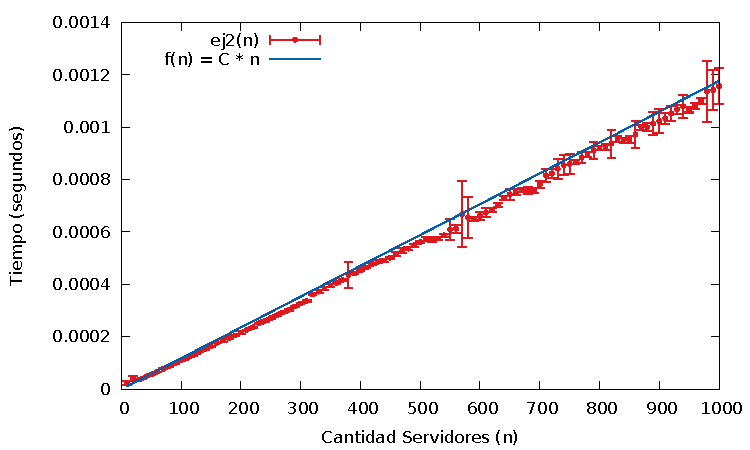
\includegraphics{imgs/ej2_1000_10_100.pdf}
\caption{Test Performance: Tiempo(s) vs Cantidad de Servidores}
\end{figure}

Notar que los tiempos de ejecución se incrementan linealmente en función de la cantidad de servidores.
 
\subsection{Preguntas Adicionales}

\textbf{1 - }  \emph{Mostrar con un contraejemplo que es posible resolver las dos partes por separado de manera óptima pero que aun así haya una solución en la que la replicación termine en menos tiempo. Comentar posibles soluciones al problema.}\\

Podemos ver el siguiente ejemplo, supongamos que tenemos el grafo: 

\begin{figure}[H]
\centering
\def\svgwidth{140 pt}
\input{imgs/ejemploEj2_b.pdf_tex}
\end{figure}

Se puede ver que tenemos dos árboles generadores mínimos. 

\begin{figure}[H]
\centering
\def\svgwidth{200 pt}
\input{imgs/ejemploEj2_b2.pdf_tex}
\end{figure}

Nuestro procedimiento devuelve el árbol de la izquierda. No obstante, el de la derecha tiene un tiempo de broadcast mejor más chico.  

\textbf{2 - }  \emph{¿Cómo se debe modificar la solución si en lugar de transmitir por broadcast se lo hace por multicast, es decir, se debe mandar un paquete a cada destino, sin hacer copias?}\\

Habría que modificar el ejercicio 2-B únicamente. En la versión del problema que funciona por broadcast nos importa buscar el nodo que garantice que el tiempo de broadcast total sea el menor posible. Si lo hacemos por multicast entonces tenemos que enviar el dato a todos los nodos, una vez a cada uno. Esto significa recorrer todos los caminos del árbol posibles para llegar hasta cada nodo. Deberíamos modificar la solución del ejercicio para que esta recorra todos los caminos hasta todos los nodos posibles, lo cual podemos hacer con una versión modificada de DFS, que guarde todos los caminos que vamos recorriendo para llegar a cada nodo.
